\let\negmedspace\undefined
\let\negthickspace\undefined
\documentclass[journal,12pt,twocolumn]{IEEEtran}
\usepackage{cite}
\usepackage{amsmath,amssymb,amsfonts,amsthm}
\usepackage{algorithmic}
\usepackage{graphicx}
\usepackage{textcomp}
\usepackage{xcolor}
\usepackage{txfonts}
\usepackage{listings}
\usepackage{enumitem}
\usepackage{mathtools}
\usepackage{gensymb}
\usepackage{comment}
\usepackage[breaklinks=true]{hyperref}
\usepackage{tkz-euclide} 
\usepackage{listings}
\usepackage{gvv}                                        
\def\inputGnumericTable{}                                 
\usepackage[latin1]{inputenc}                                
\usepackage{color}                                            
\usepackage{array}                                            
\usepackage{longtable}                                       
\usepackage{calc}                                             
\usepackage{multirow}                                         
\usepackage{hhline}                                           
\usepackage{ifthen}                                           
\usepackage{lscape}
\usepackage{caption}
\newtheorem{theorem}{Theorem}[section]
\newtheorem{problem}{Problem}
\newtheorem{proposition}{Proposition}[section]
\newtheorem{lemma}{Lemma}[section]
\newtheorem{corollary}[theorem]{Corollary}
\newtheorem{example}{Example}[section]
\newtheorem{definition}[problem]{Definition}
\newcommand{\BEQA}{\begin{eqnarray}}
\newcommand{\EEQA}{\end{eqnarray}}
\newcommand{\define}{\stackrel{\triangle}{=}}
\theoremstyle{remark}
\newtheorem{rem}{Remark}
\begin{document}

\bibliographystyle{IEEEtran}
\vspace{3cm}

\title{10.5.2.14}
\author{EE23BTECH11003 - pranav}
\maketitle
\newpage

\bigskip


\textbf{Question}:
How many multiples of 4 lie between 10 and 250?\\
\solution
let $4n_{1}$ and $4n_{2}$ be the first and last multiples of 4 between 10 and 250 then
\begin{align}
     4n_{1}>10   \text{ and }  4n_{2}<250  \\
 \implies n_{1}>10/4\text{ and } n_{2}<250/4\\
 \therefore n_{1} \text{ and } n_{2} \in \mathbb{N}\\
\implies n_{1}=3,n_{2}=62 
\end{align}
 $\therefore$ number of multiples of 4 which lie between  10 and 250 are $62-3+1=60$ \\
considering the series to start from $n=0$ the general term
\begin{align}
X(n)=[X(0)+n\cdot d].u(n)\\
X(n)=[12+4\cdot n].u(n)
\end{align}
\begin{table}[h]
    \centering
    \begin{tabular}[12.1pt]{ |c| c| c|}
    \hline
    \textbf{Variable} & \textbf{Description} &\textbf{Value}\\ 
    \hline
    $x(n)$ & value of $x$ before runge kutta iteration & $0$ \\
    \hline 
    $y(n)$ & value of $y$ before runge kutta iteration  &$1$ \\
    \hline 
    $y(n+1)$ & value of $y$ after runge kutta iteration & $?$?\\
    \hline
   $x(n+1)$ & value of $x$ after runge kutta iteration  & $?$\\
   \hline
   $f(x,y)$ &derivative of $y$ w.r.t to $x$ & $2x+y$\\
   \hline
   $h$ & step size & $0.1$\\
   \hline
    \end{tabular}

    \caption{Variables Used}
    \label{tab:table_11.9.3.6}
\end{table}
\begin{figure}[h!]
    \centering
    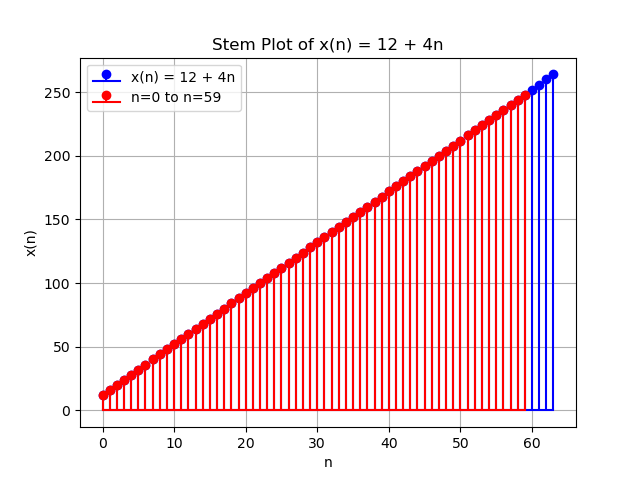
\includegraphics[width=1.1\linewidth]{figs/graph1.png}
    \caption{general term of the AP}
\end{figure}\\
applying Z transform
\begin{align}
    X(z)&= \sum_{n=-\infty}^{\infty}X(n)\cdot z^{-n}\\
   \implies X(z)&= \sum_{n=-\infty}^{\infty} [12+4\cdot n]\cdot u(n)\cdot z^{-n}\\
   \implies X(z) &=\sum_{n= 0}^{\infty} [12+4\cdot n] \cdot z^{-n}\\
   \implies X(z)&= \frac{12}{1-z^{-1}} +\frac{4\cdot z^{-1}}{(1-z^{-1})^{2}}
\end{align}
\end{document}
